\section{Expedition Findings}

\margininbox{Logbook}{W566 BFR is our bus of joy, 5.6 metres long

\textbf{Ferries:}

Out on Sat 14th July, 1345 ish, back Sun 12th August, 1100 ish.

Quotes (8-12 weeks in advance): P\&O (9 passengers): 156.25 

With Sea France: 112.00

Sea France (4 weeks in advance): 140 \textbf{BOUGHT}
\protect\mininame{Jarv}}{\logbook}

\begin{marginfigure}
\frame{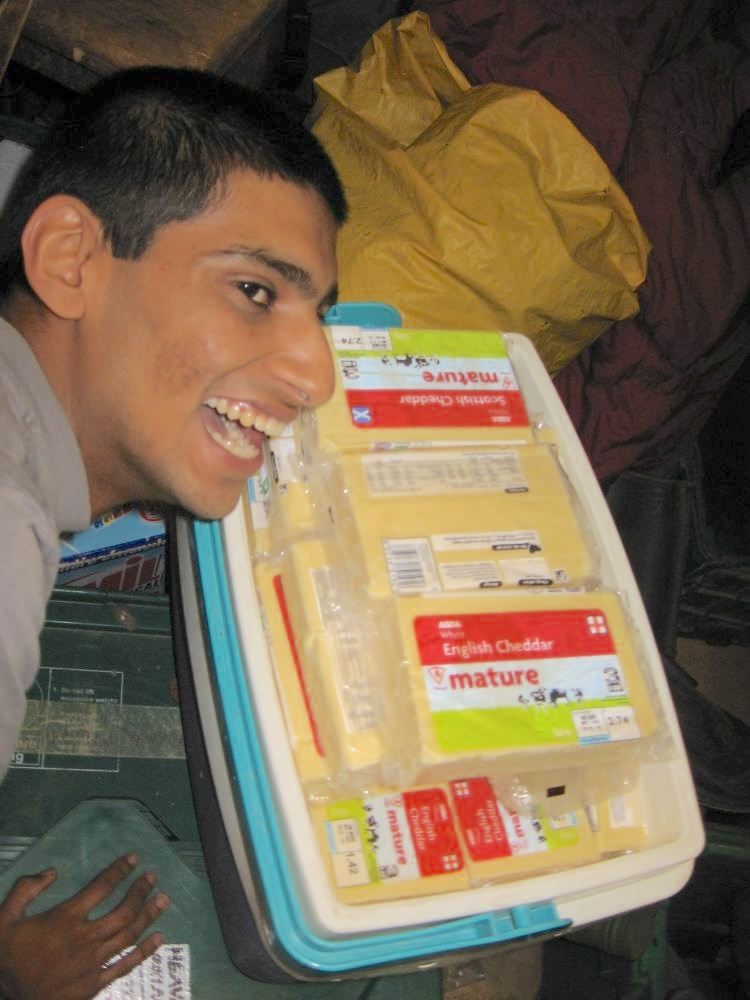
\includegraphics[width=\linewidth]{2007/expedition_findings/jarvist frost - sandeep and cheesus in stores--orig.jpg}}
\caption{Sandeep and cheesus [sic] in stores. \pic{Jarvist Frost}}
\end{marginfigure}

\subsection{\protect\passage{Plop} Goes!}

Andy and Rik pushed \passage{Plop} (the tight squeeze) onto the magnificent
\passage{Plopzilla} pitch. A field of helictites festoon the pitch down onto an
enormous boulder pile. One side of this chamber is unpushed, the other
leads to a boulder choke, as yet unpushed. \passage{Plopzilla} is 105 m
deep, penetrating from \passage{NCB} to below \passage{Exhibition road}. This
makes it the second largest pitch in the system after \passage{Silos}.

\subsection{\protect\passage{M1} \& \protect\passage{M6}}

Repushed + resurveyed. Still a lead (may need chemical persuasion) in a
window off \passage{M1}. Small extensions found in \passage{M6} - very pretty little bit of
stream formed new cave, ended in draughting bedding plane dig.

\subsection{\protect\passage{U-Bend} connected to \protect\passage{Primadona}}

Hard pushing by Sandeep and Alvin through the previously blown \passage{Enigma
squeeze} on the 40 m \passage{U-Bend} pitch has led to a connection with the \passage{Drugi Vhod}
entrance to \passage{Primadona}, gaining \passage{Primadona} an additional 57
m of height, making a cave 644 m deep. Beautiful survey accuracy - have
a look on the .3d file!

\subsection{\protect\passage{Razor Cave} survey}

Coordinated by Martin, we've started to survey \passage{Razor Cave}. 250 m
already in the book; it's a very interesting clearly fault-driven cave,
with easy access from the Razor hut.

\subsection{New caves on western edge of plateau}

\begin{pagefigure}
      \checkoddpage \ifoddpage \forcerectofloat \else \forceversofloat \fi
      \centering
              \frame{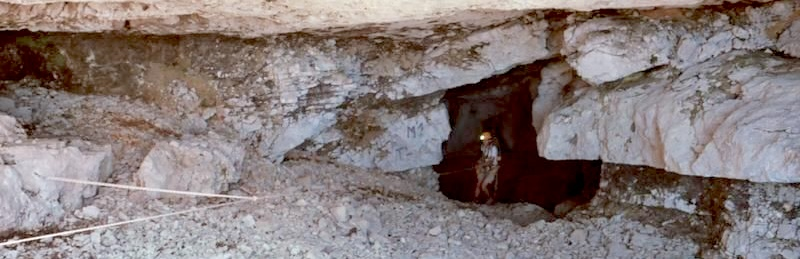
\includegraphics[width=\linewidth]{2007/expedition_findings/jarvist frost gr1 film1 -029_26--orig.jpg}} 
  \caption{The impressive \passage{M1} entrance scree slope. \pic{Jarvist Frost}}
\end{pagefigure}

\passage{Planika} (named after the Edelweiss present on the western plateau) and ``\passage{Monatip}'', found below \passage{B9}/\passage{M21} (on the western edge
of the plateau, approx 100 m north of \passage{Primadona}) and the initial pushing trips conducted. \passage{Planika}: 166 m long, 46 m deep \passage{Monatip}: 196 m long, 28 m deep.

\begin{marginfigure}
\frame{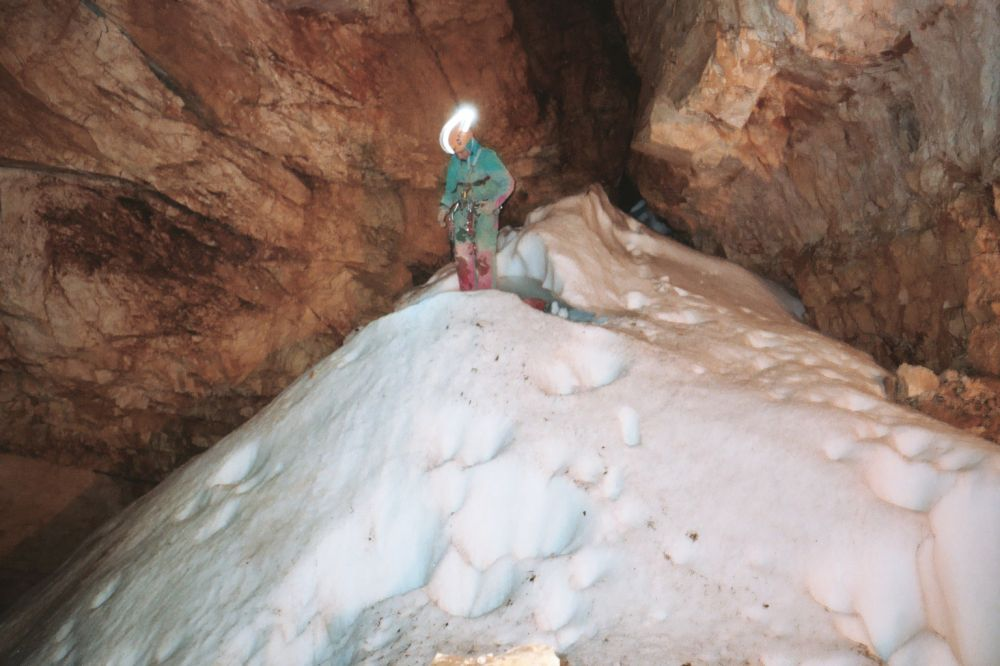
\includegraphics[width=\linewidth]{2007/expedition_findings/jarvist frost gr1 film4 -032_29--orig.jpg}}
\caption{The snow-filled first chamber of \passage{Planika Jama}. \pic{Jarvist Frost}}
\end{marginfigure}

\passage{Planika} is a high entrance (1801 m) which leads directly to a 40 m pitch to a snow plug. Climbing the snow gains another chamber with a large entrance, and a rift leading off. A very tight pitch head at the end of rift leads to a 5 m pitch which reconnects to a 20 m long snow slope. 

Digging at the bottom of this snow slope gained another snow filled chamber, with `phreatic' esque passage etched through the snow by the draught, and extremely drippy snow which I believe is certainly feeding a faithful stream, possibly the one that was found on \passage{Smer0} in \passage{Primadona}, 200 m below. 

To get to \passage{Planika}, one must conduct a 30
m abseil down a cliff, then traverse along the ledge. Extremely pretty - one gets a view across the whole of the Tolminka by day, or the lights of Italy all the way to Venice by night.

\passage{Monatip} is directly below \passage{Planika} (24 m between bottom of snow
plug and early passage), and has a very \passage{NCB}-like character -
possibly a dried river bed. It undulates along, heading into blank
mountain.

\begin{marginfigure}
\frame{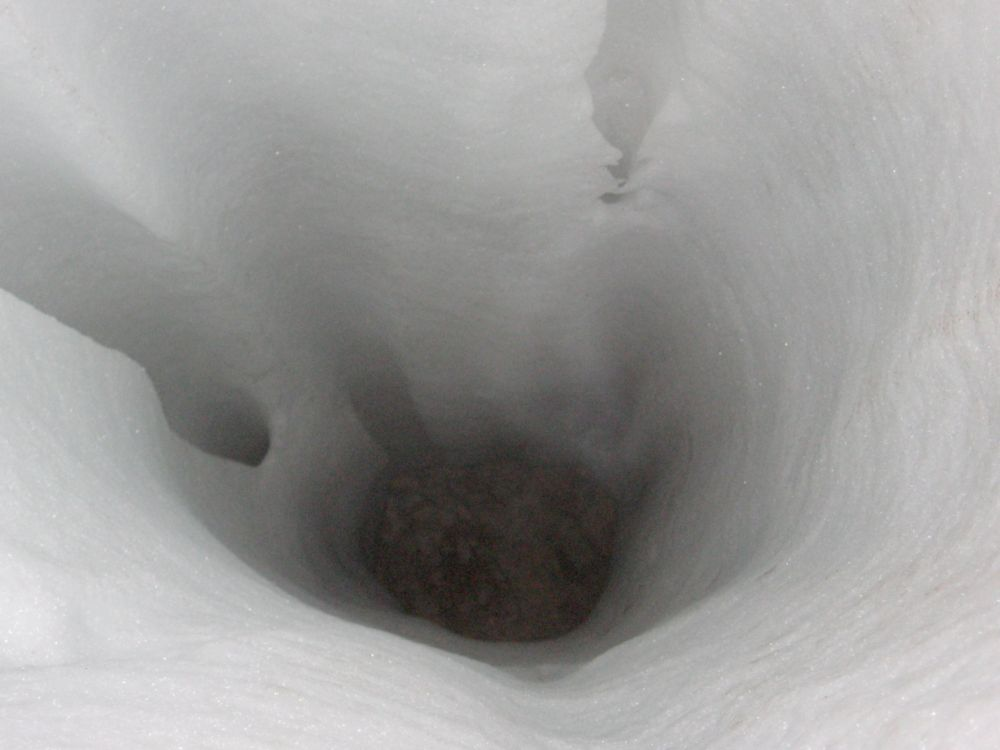
\includegraphics[width=\linewidth]{2007/expedition_findings/jarvist frost - planika first snow chamber - 8m deep hole in snow--orig.jpg}}
\caption{An 8m deep snow hole in \passage{Planika Jama}. \pic{Jarvist Frost}}
\end{marginfigure}

\begin{marginfigure}
\frame{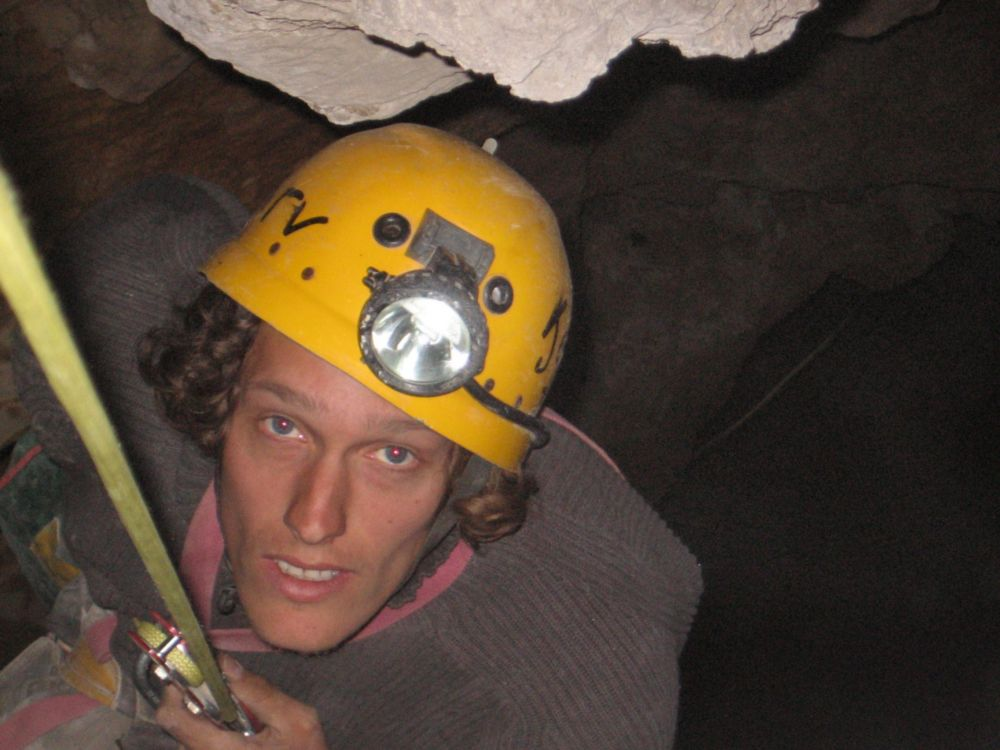
\includegraphics[width=\linewidth]{2007/expedition_findings/jana carga - jarv near rebelay entrance pitch planika--orig.jpg}}
\caption{Jarv descending near the first rebelay in \passage{Planika Jama}. \pic{Jana Čarga}}
\end{marginfigure}


\subsection{\protect\passage{Primadona} \protect\passage{Smer0}
pitch}

Initial rigging of the \passage{Smer0} pitch discovered in October 2006 was
undertaken, bolting down to about -40 m. Pitch is ongoing.
Stream was followed upstream to a tight labyrinth.

\subsection{\protect\passage{Smashed Swede}}

Stefan's climb was bolt-traversed to by Rik and Paul, gaining a window
that would appear to reconnect to \passage{Hardy} Pitch. A second look
wouldn't go amiss.

\section{Minor Caves}

\subsection{\protect\passage{East Pole} (\protect\passage{S1})}

Further work was undertaken in \passage{East Pole} {\passage{S1}). A number of promising new
holes were investigated, including \passage{E1} - a roughly 25 m deep
pitch leading to too-tight windows that require opening up.

\subsection{\protect\passage{Stag Cave}}

A cave was found within 20 m of the tents! A short pitch, rigged on
naturals, lead to a spacious chamber that was unfortunately dead.
However the presence of a large collection of bones (some crushed, but
many in very good condition) that appears to have been from a stag made
up for the disappointment!

\subsection{\protect\passage{Moth Cave}}

\begin{marginfigure}
\frame{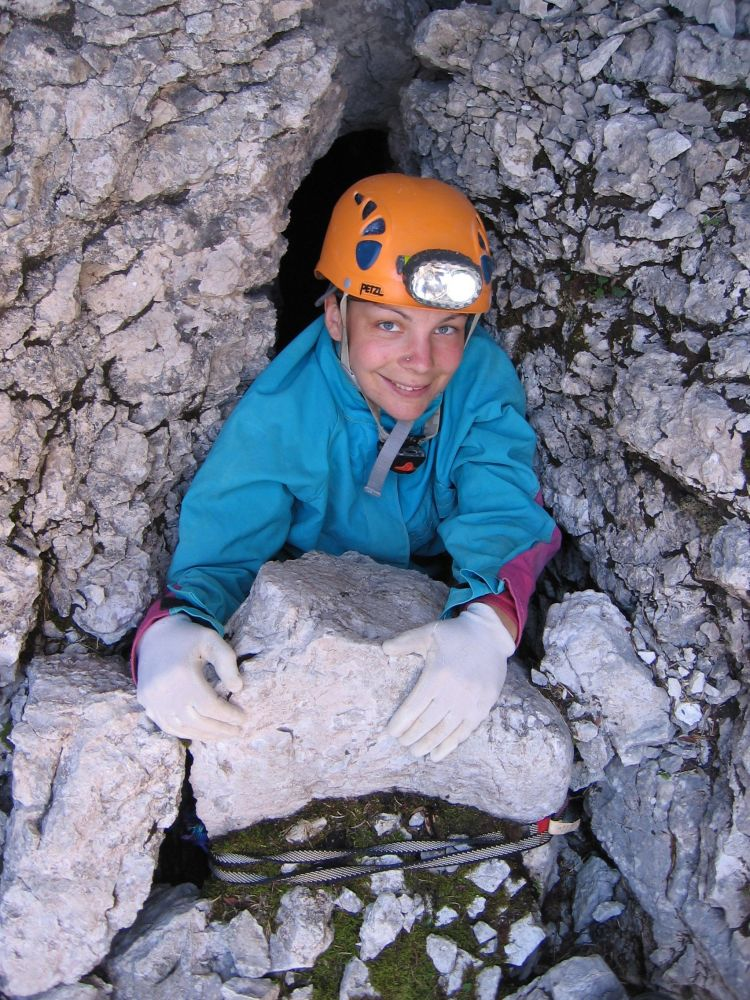
\includegraphics[width=\linewidth]{2007/expedition_findings/jarvist frost - jana entrance to e1--orig.jpg}}
\caption{Jana in the entrance to \passage{E1}. \pic{Jarvist Frost}}
\end{marginfigure}

Heroic effort was expended in the \passage{Moth Cave} dig: two extra chambers were
gained, but unfortunately only lead to yet another too-tight squeeze
requiring rock removal. Declared dead and derigged.

\subsection{\protect\passage{Hawk Cave}}

New (safe) method of gaining the cave was constructed by bolting an
abseil from the cliff-head. Most leads off chamber were found to die, a
bolt traverse was made across the pitch to find an aven where we hoped a
parallel shaft may lie. Still to be revisited - we ran out of time and
rope, and so derigged.




\name{Jarvist Frost}

\begin{pagefigure}
      \checkoddpage \ifoddpage \forcerectofloat \else \forceversofloat \fi
      \centering
              \frame{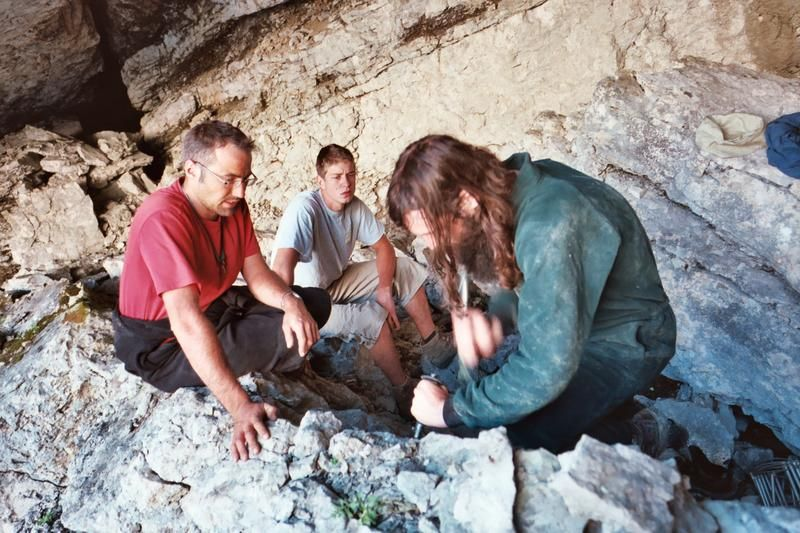
\includegraphics[width=\linewidth]{2007/expedition_findings/jarvist frost gr1 film3 -029_26--orig.jpg}} 
       \label{surface bashing}
  \caption{A surface, quite literally being bashed by James Huggett. \pic{Jarvist Frost}}
\end{pagefigure}

